\documentclass[journal]{IEEEtran}

\usepackage{amsmath,amssymb,caption,comment,enumitem,float,graphicx,microtype}
\usepackage[utf8]{inputenc}
\usepackage[T1]{fontenc}
\usepackage[margin=1in]{geometry}
\usepackage{setspace}
\usepackage{fancyhdr}
\usepackage{bm}
\pagestyle{fancy}
\fancyhf{}
\rhead{\today}

\newcommand{\N}{{\mathbb N}}
\newcommand{\Z}{{\mathbb Z}}
\newcommand{\Q}{{\mathbb Q}}
\newcommand{\R}{{\mathbb R}}
\newcommand{\C}{{\mathbb C}}
\newcommand{\F}{{\mathbb F}}
\newcommand{\E}{{\mathbb E}}
\mathchardef\hyphen="2D

\title{6.867 Homework 1}
\author{Anonymous Authors}

\begin{document}

\maketitle
\thispagestyle{fancy}

\section{Implementing Gradient Descent}


In any gradient descent algorithm, the main hyperparameters we have to tune are the initial point we start the gradient descent from, the step size, and the convergence criteria. 

\begin{itemize}

\item An incorrect initial guess could lead to getting stuck at a local min without ever reaching the global minumum
\item A step size that is too large can shoot past the minumum or go back and forth without ever reaching the critical point. Conversely, a step size that is too small can make the algorithm take far too long to converge.
\item A convergence criteria that is too lax can result in a sub-optimal stopping point, while a convergence criteria that is too strict can result in the algorithm taking too long.

\end{itemize}

For each of the three parameters, we can see how varying the parameters changes the gradient descent for both of the provided functions (the Gaussian and the bowl).

Default parameters are: 

\begin{itemize}

\item Starting Point: (0,0)
\item Step Size: 0.01
\item Convergence Criteria: Difference between consecutive objective function values is less than $10^{-10}$, max of 20,000 iterations

\end{itemize}

\section{Linear Basis Function Regression}

\subsection{Closed-form Solution with Polynomial Basis}
% Replicate plots
Consider the basis function $$\Phi_M(x) = [\phi_0(x), \dots, \phi_M(x)],$$ where $\phi_k(x) = x^k$. Applying $\Phi_M$ to $\mathbf{X}$ gives the desired basis change, so we have the generalized linear model $$\mathbf Y = \Phi_M(\mathbf X) \cdot \bm \beta + \bm \epsilon,$$ which has the close-form solution $$\hat{\bm \beta} = (\Phi_M(\mathbf X)^T \Phi_M(\mathbf X))^{-1} \Phi_M(\mathbf X)^T \mathbf Y,$$
where $\hat{\bm \beta}$ is the maximum-likelihood estimator of the regression coefficients.

We ran regressions on the data using a few different degrees $(M = 0, 1, 3, 10)$.\footnotemark\ Below are plots of the resulting polynomial functions, compared to the given data and the true function:

\footnotetext{See the Appendix for the numerical values of the weights.}

\begin{figure}[H]
  \centering
  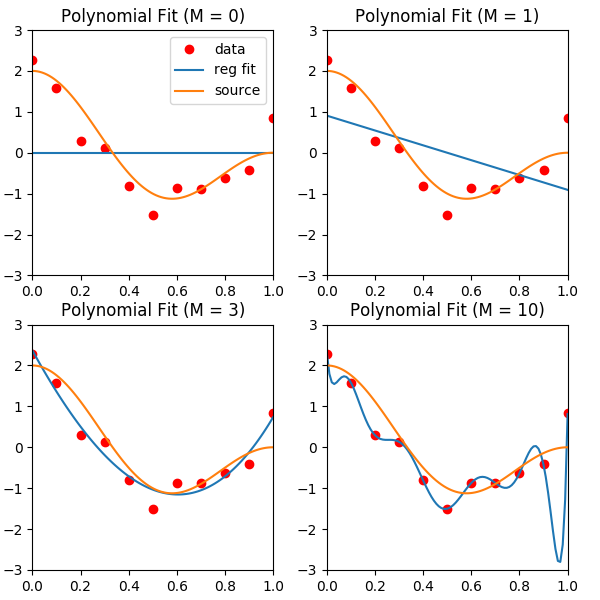
\includegraphics[width = 3.15in]{../P2/fig/part_1.png}
  \caption{M-Degree Polynomial Fit (M = 0, 1, 3, 10)}
\end{figure}

\subsection{Gradient Descent Solution with Polynomial Basis}
% Minimize SSE with Batch GD and SGD

\subsection{Closed-form Solution with Cosine Function Basis}

\section{Ridge Regression}

\section{Sparsity and Lasso}

\section{Appendix}
% Coefficients in 2.1

\end{document}